\subsection{Planar Graphs and their Properties}

\begin{definition}[Planarity]
    A graph is planar if some embedding of it onto the plane has no edge intersections.
\end{definition}

\begin{center}
    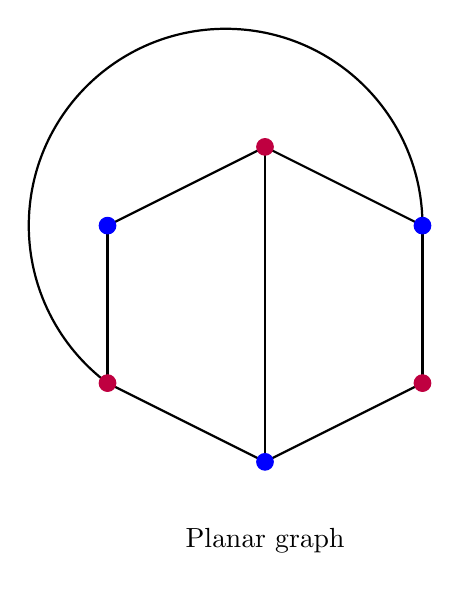
\begin{tikzpicture}
        \draw[black, thick] (0,1) -- (2,0);
        \draw[black, thick] (2,0) -- (4,1);
        \draw[black, thick] (4,1) -- (4,3);
        \draw[black, thick] (4,3) -- (2,4);
        \draw[black, thick] (2,0) -- (2,4);
        \draw[black, thick] (2,4) -- (0,3);
        \draw[black, thick] (0,3) -- (0,1);
        \draw[black, thick] (4,3) arc (0:270-asin(3/5):2.5);
        \filldraw[purple] (0,1) circle (3pt);
        \filldraw[purple] (4,1) circle (3pt);
        \filldraw[purple] (2,4) circle (3pt);
        \filldraw[blue] (0,3) circle (3pt);
        \filldraw[blue] (4,3) circle (3pt);
        \filldraw[blue] (2,0) circle (3pt);
        \node at (2,-1,0) {Planar graph};
    \end{tikzpicture}
    \hspace{2cm}
    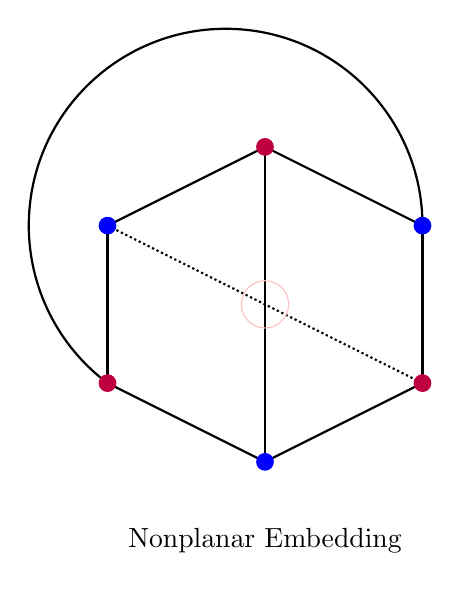
\begin{tikzpicture}
        \draw[black, thick] (0,1) -- (2,0);
        \draw[black, thick] (2,0) -- (4,1);
        \draw[black, thick] (4,1) -- (4,3);
        \draw[black, thick] (4,3) -- (2,4);
        \draw[black, thick] (2,0) -- (2,4);
        \draw[black, thick] (2,4) -- (0,3);
        \draw[black, thick] (0,3) -- (0,1);
        \draw[densely dotted, black, thick] (0,3) -- (4,1);
        \draw[black, thick] (4,3) arc (0:270-asin(3/5):2.5);
        \filldraw[purple] (0,1) circle (3pt);
        \filldraw[purple] (4,1) circle (3pt);
        \filldraw[purple] (2,4) circle (3pt);
        \filldraw[blue] (0,3) circle (3pt);
        \filldraw[blue] (4,3) circle (3pt);
        \filldraw[blue] (2,0) circle (3pt);
        \draw[pink] (2,2) circle (0.3);
        \node at (2,-1,0) {Nonplanar Embedding};
    \end{tikzpicture}
\end{center}